\documentclass{SGGW-thesis}
\usepackage{xcolor,amsfonts}
\NewCommandCopy{\amshbar}{\hbar}

\INZYNIERSKAtrue
\WZIMtrue

\title{Wykorzystanie technologii webowych i języka Python do stworzenia aplikacji edukacyjnej z mechaniki kwantowej}
\Etitle{Utilizing web technologies and Python language to create quantum physics educational application}

\author{Adrian Rostek}
\album{205860}
\thesis{Praca dyplomowa na kierunku:}
\course{Informatyka}
\promotor{dr. Andrzeja Zembrzuskiego}
\pworkplace{Instytut Informatyki Technicznej\\Katedra Systemów Informatycznych}

\usepackage{hyperref}
\usepackage{amsmath}
\usepackage{float}

\begin{document}
\maketitle
\statementpage
\abstractpage
{Wykorzystanie technologii webowych i języka Python do stworzenia aplikacji edukacyjnej z mechaniki kwantowej}
{...Treść streszczenia...}
{Edukacja, Fizyka kwantowa, Funkcja falowa, Wizualizacja}
{Utilizing web technologies and Python language to create quantum physics educational application}
{...Treść angielskiego streszczenia...}
{Education, Quantum physics, Wave function, Visualization}


{
  % Spis treści może być złożony z pojedynczą interlinią, np. jeśli jedna linia wychodzi na następną stronę.
  % W przeciwnym razie spis treści wstawić bez powyższego rozkazu i klamry.
  \doublespacing
  \tableofcontents
}

\startchapterfromoddpage % niezależnie od długości spisu treści pierwszy rozdział zacznie się na nieparzystej stronie

\chapter{Wstęp}
Stworzenie mechaniki kwantowej okazało się niezwykle istotne dla dzisiejszej cywilizacji. Zawdzięczamy jej m.in. tranzystory oraz reaktory jądrowe, bez których ciężko wyobrazić sobie dzisiejszą energetykę \cite{nuclear-stats}. Mimo to jest to bardzo nieintuicyjny i przez większość ludzi niezrozumiały dział fizyki \cite{fiz atom}. Na temat ten napisane zostały liczne publikacje \cite{fiz atom} \cite{mechanika kwant} \cite{fiz kwant}, jednak profesjonalny język i matematyka wyższa mogą sprawić dużo trudności w zrozumieniu nawet podstawowych konceptów tej teorii.

	\section{Cel i motywacja pracy}
	Celem pracy jest stworzenie aplikacji, która ma ułatwić naukę zagadnień z zakresu mechaniki kwantowej. Zagadnienia przedstawiane są w interaktywny sposób celem podtrzymania uwagi i zainteresowania tym nietrywialnym tematem. Osiągnięte to zostało poprzez wykorzystanie szeregu prezentacji wizualnych, na których efekt końcowy bezpośredni wpływ ma użytkownik, jednocześnie stosując samouczek, który te efekty odpowiednio tłumaczy.
	
	Osobiście temat mechaniki kwantowej uważam za niezwykle ciekawy, więc napisanie tej pracy motywowane jest chęcią poszerzenia swojej wiedzy w tym obszarze, jak i zastosowaniu nabytej wiedzy informatycznej w stworzeniu praktycznego narzędzia. Za interesujące również uważam symulację funkcji falowej w przeciwieństwie do przypatrywania się statycznym jej wykresom na papierze czy w plikach pdf. Aplikacja kierowana jest do osób chcących nauczyć się wstępnych zagadnień mechaniki kwantowej, jednak bez konieczności sięgania po profesjonalną literaturę. Do pełnego zrozumienia wszystkich zagadnień potrzebna jest znajomość podstaw matematyki wyższej, jednak nawet bez tej wiedzy użytkownik może wynieść z aplikacji dużo nowych informacji. Może ona być więc użyteczna nie tylko dla studentów fizyki, ale też osób ciekawiących się tym tematem.
	\section{Tematyka i struktura pracy}
	Aplikacja przytacza kontekst historyczny dziedziny fizyki jaką jest mechanika kwantowa jak i opisuje korpuskularno-falową naturę cząstek. Główna część jednak skupia się na typowych rozwiązaniach równania Schrödingera niezależnego od czasu, a dokładniej dla:
	\begin{itemize}
	\item cząstki swobodnej,
	\item nieskończonej studni potencjału,
	\item skończonej studni potencjału,
	\item progu potencjału,
	\item bariery potencjału.
	\end{itemize}
	
	Wytłumaczone są też zjawiska tunelowe i skwantowanych stanów energetycznych jako konsekwencja dotychczas przyswojonych zagadnień. Są to często omawiane zagadnienia w podręcznikach wprowadzających do mechaniki kwantowej \cite{fiz atom} \cite{mechanika kwant} \cite{fiz kwant}, ponieważ przypadki te dobrze obrazują istotę funkcji falowej.
	
	W rozdziale drugim opisane zostały zastosowane technologie, charakterystyka ich działania oraz wytłumaczone zostało czym motywowany był wybór akurat ich do stworzenia aplikacji.
	
	W rozdziale trzecim szerzej wyjaśniony został dokładny zakres zagadnień zawartych w aplikacji oraz uzasadniony został powód upraszczania niektórych z nich i poświęcanie większej uwagi na pozostałe.
	
	Rozdział czwarty skupia się na technicznych aspektach budowy aplikacji, omawia szczegóły implementacji wymaganych rozwiązań i problemy z tym związane. Omówione również zostały ograniczenia zastosowanych technologii, jak i otwartość aplikacji na rozwój.
	
	W rozdziale piątym zaprezentowane są zrzuty ekranu z działania aplikacji, wytłumaczona zostaje budowa i działanie interfejsu oraz jak spełnione zostało wstępne wymaganie aplikacji, czyli ułatwianie nauki.
	
	Pracę kończy rozdział zawierający podsumowanie i wnioski.
	
	
\chapter{Wykorzystane technologie}
	\section{Popularne technologie webowe -- HTML, CSS i TypeScript}
	
	\section{Biblioteki Chart.js i MathJax}
	Chart.js jest aktualnie najpopularniejszą biblioteką, do tworzenia wykresów w języku JavaScript \cite{chartjs}, z bogatą dokumentacją i liczbą funkcji. Co było dla mnie najważniejsze przy jej wyborze, to szybka i czytelna konfiguracja wykresów liniowych. Biblioteka daje wiele możliwości dostosowywania wyglądu generowanych wykresów jak i ich dynamicznej edycji po wygenerowaniu.
	
	Kolejnym ważnym aspektem jest dostępność wbudowanych w bibliotekę typów, co umożliwia stosowanie jej w języku TypeScript, korzystając z zalet jakie wprowadza do języka JavaScript. We wstępnych wersjach aplikacji wykorzystywałem bibliotekę Plotly, jednak typy, pomimo że dla niej dostępne, nie są w pełni dopracowane, co wymuszało wyłączenie reguły no-explicit-any w konfiguracji języka TypeScript dla projektu. W konsekwencji tworzyło to sytuację, w której istniało ryzyko tworzenia kodu o słabym typowaniu, co w dłuższej perspektywie mogłoby sprzyjać pojawianiu się w kodzie błędów związanych z typami.
	
	Drugą użytą biblioteką, jednak nie stosowaną bezpośrednio w kodzie TypeScript, a w plikach HTML, jest MathJax. Umożliwia ona umieszczanie zaawansowanych formuł matematycznych, na stronach pisanych w języku HTML \cite{mathjax}, co było konieczne dla poruszanych w aplikacji zagadnień. Formuły umieszczane są pomiędzy znakami \$\$ \$\$ lub \textbackslash( \textbackslash), a ich składnia, pomimo że trochę odmienna, jest bardzo zbliżona do popularnego LaTeX'a. Wszelkie odstępstwa od LaTeX'a można szybko zweryfikować dzięki szczegółowej dokumentacji. Istotny jest również fakt, że nie jest wymagane umieszczanie całej biblioteki lokalnie w projekcie, co zajmowałoby dosyć dużo miejsca. Zamiast tego wystarczy umieścić odpowiednią adnotację w pliku HTML, aby pobrać niezbędne zasoby z internetu.
	
	\section{Język Python}
	Python pomimo, że znacząco wolniejszy od wielu innych języków programowania (str. 2 w  \cite{Python}), posiada bogatą kolekcję bibliotek do przetwarzania danych i obliczeń matematycznych m.in. NumPy, SciPy i SymPy. Biblioteki te najczęściej napisane w C lub Fortranie, są już z kolei znacznie szybsze od czystego Pythona (str. 2 w \cite{Python}). Charakterystyczna jest też jego przejrzysta składnia, zawierająca dużo lukru składniowego(str. 418 w \cite{Python}).
	
	Głównymi powodami, dla których użyłem języka Pythona, jest właśnie dostępność bibliotek, a szczególnie SymPy oraz wbudowana obsługa liczb zespolonych. Co prawda do rachunku na liczbach zespolonych nie musiałem sięgać po drugi, zaraz po języku TypeScript, język programowania, jednak składnia Pythona jest w tym zastosowaniu znacznie bardziej zwięzła. Biblioteka SymPy z kolei nie została wykorzystana w żadnym miejscu w implementacji aplikacji, więc może się wydać nietypowym argumentem za wyborem języka, jednak tłumaczę ten wybór dokładniej w kolejnym akapicie. 
	
	SymPy jest biblioteką umożliwiającą obliczenia w matematyce symbolicznej \cite{sympy}, co najważniejsze pozwala na znajdowanie analitycznych rozwiązań dla równań różniczkowych. W mojej opinii umożliwia to łatwiejszy rozwój aplikacji i wzbogacenie jej o bardziej zaawansowane przypadki ruchu cząstki w przestrzeni.
	
	Dostępność Matplotlib i podobnych bibliotek szkicujących umożliwia rysowanie wykresów do wizualizacji danych, wymagając przy tym bardzo małej ilości kodu, co może okazać się niezwykle przydatne przy sprawdzaniu poprawności implementacji obliczeń bardziej złożonych wzorów matematycznych. Przy pisaniu pracy niejednokrotnie z takiej możliwości skorzystałem, na co najczęściej potrzebne były 3-4 linie kodu.
	
	\section{Framework Tauri}
	Za pomocą Tauri możliwe jest tworzenie aplikacji desktopowych, wykorzystując przy tym technologie webowe. W przeciwieństwie do rozwiązań takich jak Electron \cite{electron}, aplikacje tworzone przy użyciu Tauri zajmują znacznie mniej miejsca oraz potrzebują mniej zasobów komputera do działania. 
	Dodatkowym atutem jest możliwość korzystania z interpretera Pythona, zainstalowanego na komputerze użytkownika. Standardowe aplikacje webowe w przeglądarce również umożliwiają wykonywanie skryptów Pythona, za pomocą interpretera skompilowanego do WebAssembly \cite{WebAssembly Python}, drugiego po JavaScript języka programowania obsługiwanego przez popularne przeglądarki \cite{browser langs}. Jest to niestety rozwiązanie stosunkowo nowe i we wczesnej fazie rozwoju \cite{python-webassembly}.
	
\chapter{Podstawy teorytyczne}
	\section{Zagadnienia matematyki wyższej}
	Niewątpliwie matematykę, a szczególnie rachunek różniczkowy, można nazwać językiem fizyki. Do opisu zawartych w pracy zagadnień fizycznych, wymagana jest pewna znajomość zagadnień matematyki wyższej.

	Liczby zespolone są nadzbiorem liczb rzeczywistych, wzbogaconym o jednostkę urojoną $i$ \cite{liczby zespolone}definiowaną jako: 
	
	\begin{equation}
	i^2=-1.
	\end{equation}
	
	Dowolną liczbę zespoloną możemy więc zapisać w postaci algebraicznej, będącej sumą części rzeczywistej i urojonej, tj. będącej rzeczywistą wielokrotnością jednostki urojonej:
	
	\begin{equation}
	z = a+bi,
	\end{equation}
	gdzie
	$z \in \mathbb{C}$,
	$a \in \mathbb{R}$,
	$b \in \mathbb{R}$.\\
	
	Do graficznego opisu liczby zespolonej poza osią rzeczywistą, potrzebna jest dodatkowa, pionowa oś urojona. Liczba zespolona może być przedstawiona jako punkt o współrzędnych $a$ i $b$ w kartezjańskim układzie współrzędnym. Moduł liczby $z$ definiowany jako odległość tego punktu od środka układu współrzędnych, można więc obliczyć stosując twierdzenia Pitagorasa:
	
	\begin{equation}
	|z| = \sqrt{a^2+b^2},
	\end{equation}
	
	gdzie:
	
	$ z = a + bi$,
	
	$z \in \mathbb{C}$,
	$a \in \mathbb{R}$,
	$b \in \mathbb{R}$.\\
	
	Inną postacią liczby zespolonej jest postać wykładnicza, przedstawiana jako:
	
	\begin{equation}
	z = |z|e^{i\phi},
	\end{equation}
	
	gdzie:
	
	$z \in \mathbb{C}$,
	
	$e$ -- podstawa logarytmu naturalnego,
	
	$i$ -- jednostka urojona,
	
	$\phi$ -- kąt pomiędzy osią części rzeczywistej, a ramieniem poprowadzonym ze środka układu współrzędnych do liczby $z$.\\
	
	Szczegóły funkcji falowej $\psi$ wytłumaczone są w dalszej części pracy, jednak na szczególną uwagę zasługuje wartość kwadratu jej modułu, określająca gęstość prawdopodobieństwa znalezienia cząstki w danym położeniu. Oznacza to, że prawdopodobieństwo znalezienia cząstki w jednowymiarowym obszarze $[x_1, x_2]$ będziemy wyznaczać jako:
	\begin{equation}
	P(X) = \int\limits_{x_2}^{x_1} |\psi(x)|^2dx,
	\end{equation}
	
	gdzie:
	
	$X$ -- zdarzenie losowe, że cząstka znajduje się w obszarze,
	
	$x_1, x_2$ -- początek i koniec obszaru.\\ 	
	
	Równanie różniczkowe to równanie funkcyjne zawierające pochodne nieznanej funkcji. Znajdowanie rozwiązań takich równań znacząco wykracza poza wiedzę wymaganą do zrozumienia omawianych zagadnień fizycznych, więc nie będzie do tego przywiązywana szczególna uwaga. Wybrany zakres zagadnień wymaga jedynie zapamiętania rozwiązania jednego rodzaju równań:
	
	\begin{equation}
	f''(x)+K^2f(x)=0 \;\Longleftrightarrow f(x)\; = Acos(Kx) + Bsin(Kx),
	\end{equation}

	gdzie:
	
	$f(x) \; i \; f''(x)$ -- funkcja i jej pochodna względem zmiennej x,

	$K \in \mathbb{C}$,
		
	$A \in \mathbb{C}, B \in \mathbb{C}$ -- stałe wyznaczane z warunków brzegowych.
	
	

	Warto zaznaczyć, że pomimo tego, że zagadnienia te są niezbędne do pełnego zrozumienia mechaniki kwantowej, nawet bez tej wiedzy użytkownik aplikacji może dowiedzieć się o tym, jak nieintuicyjnie zachowują się cząstki.
	\section{Falowa natura materii}
	Wyjaśnione przez Alberta Einsteina zjawisko fotoelektryczne ukazało, że światło zachowuje się nie tylko jak fala, ale też jak cząstką \cite{foto-ele}. Nośnik światła przekazywał energię porcjami -- kwantami przez co wprowadzone zostało pojęcie fotonu jako cząstki światła.
	
	 Jako konsekwencja tego odkrycia Louis de Broglie zapostulował, że cząstki materii, takie jak elektron, muszą podzielać falowe zachowanie fotonów. Korzystając z pracy Einsteina określił długość tych fal \cite{matter-wave}, zwanych falami materii, wzorem:
	 
	 \begin{equation}
	 \lambda=\frac{h}{p},
	 \end{equation}
	
	 
	 gdzie:
	 
	 $\lambda$ -- długość fali materii cząstki,
	 
	 $h$ -- stała Plancka,
	 
	 $p$ -- pęd cząstki.\\
	 
	 Dzięki falom materii możemy wyjaśnić m.in. sposób rozchodzenia się elektronów np. przez siatkę dyfrakcyjną, co jest niemożliwe przy przyjęciu elektronów jako kul lub punktów w przestrzeni.
	 
	 Dokładniejszego opisu tych fal dokonał Erwin Schrödinger proponując równanie funkcji falowej $\psi$ o zespolonym zbiorze wartości. 
	 
	\section{Równanie Schrödingera}
	Funkcja falowa stanowi fundament zagadnień poruszanych w aplikacji. Wynika to z faktu, że jest ona niezbędna do opisu ruchu dowolnej cząstki. Erwin Schrödinger zawarł funkcje falową w równaniu nazwanym od jego nazwiska równaniem Schrödingera \cite{schrodinger-equation}.  Jeżeli skupimy się na odizolowanych układach fizycznych tj. takich, które nie oddziaływują z otoczeniem, rozwiązać należy równanie Schrödingera niezależne od czasu o postaci:
	\begin{center}
	\begin{equation}
		-\frac{\amshbar}{2m} \frac{d^2\psi(x)}{dx^2} + V(x)\psi(x) = E\psi(x),
	\end{equation}
	\end{center}
	gdzie:
	
	$\amshbar$ -- zredukowana stała Plancka,
	
	$\psi(x)$ -- fukcja falowa w położeniu $x$,
	
	$E$ -- energia całkowita ciała,
	
	$V(x)$ -- potencjał w położeniu, $x$
	
	$m$ -- masa ciała\\
	
	Wartość funkcji falowej $\psi(x)$ nie posiada fizycznej interpretacji, do tego potrzebny jest kwadrat jej modułu, który określa gęstość prawdopodobieństwa znalezienia cząstki w położeniu $x$. 
	\section{Znajdowanie równania funkcji falowej}
	Określenie położenia cząstki wymaga od nas rozwiązania równania Schrödingera, w którym będziemy mieli określoną funkcję $V(x)$. Rozwiązanie szczegółowe tego równania spełniać muszi warunki początkowe, mogące wynikać m.in. z normowania gęstości prawdopodobieństwa. Poza warunkami początkowymi, konieczne będzie też spełnienie warunków brzegowych tj. ciągłości $\psi(x)$ oraz, w zagadnieniach bez nieskończonego potencjału, ciągłości jej pochodnej. Ważne jest również, że tylko skończone wartości $\psi(x)$ mają fizyczny sens \cite{fiz atom}.
	
	\section{Cząstka swobodna}
	Zanim zajmiemy się bardziej złożonymi przykładami, sprawdźmy jaką postać przyjmuje $\psi$ dla cząstki swobodnej, tj. o zerowej energii potencjalnej $V(x)$, która porusza się w stronę dodatnich wartości $x$. Otrzymujemy równanie 
	\begin{equation}\label{eqn:free-particle-schrodigner}
	\frac{d^2\psi}{dx^2}+k^2\psi=0,
	\end{equation}
gdzie
	\begin{equation}
	k=\frac{1}{\amshbar}\sqrt{2mE}.
	\end{equation}
Rozwiązanie ogólne ma więc postać
	\begin{equation}\label{eqn:free-particle-gen-solution}
	\psi(x)=Ae^{ikx} + Be^{-ikx},
	\end{equation}
gdzie stała $B$ musi być równa 0, ponieważ drugi wyraz opisuje falę poruszającą się w stronę ujemnych wartości $x$. Finalnie równanie przyjmuje postać:
	\begin{equation}\label{eqn:free-particle-solution}
	\psi(x) = Ae^{ikx},
	\end{equation}
w którym stałą $A$ można wyznaczyć jeśli chciałoby się znormalizować gęstość prawdopodobieństwa $|\psi|^2$, na określonym obszarze. Widać jednocześnie, że gęstość prawdopodobieństwa jest jednolita w całym takim obszarze.
	
	\section{Nieskończona studnia potencjału}
	Zaczynając od przypadku cząstki poruszającej się w nieskończonej studni potencjału o szerokości $a$, dzielimy zagadnienie na trzy obszary. Otrzymujemy obszar I, gdzie x$\in\left(-\infty,-\frac{a}{2}\right>$, obszar II, gdzie x$\in\left<-\frac{a}{2}, \frac{a}{2}\right)$ oraz obszar III, gdzie x$\in\left<\frac{a}{2}, +\infty\right)$. W obszarach I i III potencjał jest nieskończony, więc jeśli $\psi\neq0$ to $\frac{d^2\psi}{dx^2}$ musi być nieskończone, jednak nie ma to fizycznego sensu, więc $\psi$ musi być równe 0 w tych obszarach. Dla obszaru II otrzymujemy równanie \ref{eqn:free-particle-schrodigner} oraz rozwiązanie \ref{eqn:free-particle-gen-solution}. Na potrzebę tego przypadku rozwiązanie przekształcamy na równanie
	\begin{equation}
	\psi(x) = A\sin(kx) + B\cos(kx),
	\end{equation}
mając na uwadze, że współczynniki A i B nie są równe tym z równania \ref{eqn:free-particle-gen-solution}. Ciągłość $\psi$ pomiędzy obszarami jest możliwa tylko jeśli funkcja ta będzie równa 0 na granicach studni, co jest możliwe tylko jeśli $A=0$ lub $B=0$, a szerokość studni $a$ jest całkowitą wielokrotnością długości tej fali. Zależność tę można zapisać jako
	\begin{equation}
	ka=n\pi, \;\;\textrm{gdzie}\;\;\ n\in\{1, 2, 3...\}.
	\end{equation}
Rozwiązaniem jest więc
	\begin{equation}\label{eqn:well-inside-sol}
	\begin{split}
		&\psi = Asin(kx) \;\;\ \textrm{dla} \;\;\ n\in\{2, 4, 6...\}, \\
		&\psi = Bcos(kx) \;\;\ \textrm{dla} \;\;\ n\in\{1, 3, 5...\},
	\end{split}
	\end{equation}

	\section{Skończona studnia potencjału}
	W przypadku studni skończonej postępujemy bardzo podobnie dzieląc zagadnienie na trzy obszary, jednak przyjmujemy, że potencjał wynosi 0 dla obszarów I i III oraz $-V_0$ dla obszaru II. Jako $W$ oznaczymy energię wiązania tj. dodatnią wartość wymaganą do uwolnienia cząstki z studni. W obszarze II równanie Schrödingera znowu przyjmie postać \ref{eqn:free-particle-schrodigner} z rozwiązaniem \ref{eqn:well-inside-sol}, z tą różnicą że:
	\begin{equation}\label{eqn:k-fi-well}
	k=\frac{1}{\amshbar}\sqrt{2m(V_0-W)},
	\end{equation}
Dla obszarów I i III równanie zapiszemy jako
	\begin{equation}
	\frac{d^2\psi}{dx^2}-\gamma^2 \psi = 0,
	\end{equation}
gdzie
	\begin{equation}\label{eqn:gamma-fi-well}
	\gamma = \frac{1}{\amshbar}\sqrt{2mW},
	\end{equation}
co daje rozwiązanie ogólne
	\begin{equation}
	\psi_{I,III}= Ce^{\gamma x} + De^{-\gamma x}
	\end{equation}
Celem znalezienia dozwolonych wartości $k$ dopasowujemy na granicach obszarów pochodne logarytmiczne:
	\begin{equation}
	\frac{1}{\psi_I}\frac{d\psi_I}{dx} = \frac{1}{\psi_{II}}\frac{d\psi_{II}}{dx}
	\;\; \textrm{w}\;\; 
	x=-\frac{a}{2}
	\end{equation}
oraz
	\begin{equation}
	\frac{1}{\psi_{II}}\frac{d\psi_{II}}{dx} = \frac{1}{\psi_{III}}\frac{d\psi_{III}}{dx}
	\;\; \textrm{w} \;\;
	x=\frac{a}{2}.
	\end{equation}
Z obydwu równań otrzymujemy te same wnioski:
	\begin{equation}\label{eqn:fi-well-k-gamma}
	\begin{split}
	\gamma = k \cot\left(-\frac{ka}{2}\right)\;\; \textrm{dla} \;\; B = 0,\\
	\gamma = -k \tan\left(-\frac{ka}{2}\right)\;\; \textrm{dla} \;\; A = 0.
	\end{split}
	\end{equation}
Są to warunki konieczne do spełnienia, aby otrzymać poprawny wzór funkcji $\psi$.
Zarówno we wzorach na $k$ jak i $\gamma$ znajduje się wartość energii wiązania $W$, więc zagadnienie sprowadza się do znalezienia takich wartości $W$, aby powyższe warunki były spełnione. Nie jest to problem dający się w łatwy sposób rozwiązać analitycznie, jednak pokazuje, że dla skończonej studni też istnieją pewne dyskretne stany energetyczne cząstki. W rozdziale czwartym szerzej opisałem znajdowanie tych wartości metodą numeryczną.

	\section{Próg potencjału}
	Prostokątnym progiem potencjału nazwiemy sytuację w której w punkcie wartość energii potencjalnej rośnie z $0$ do jakiejś wartości oznaczonej $V_0$. Przyjmując, że próg potencjału znajduje się w punkcie $x = 0 $, możemy zapisać:
	\begin{equation}
	\begin{split}
		&V(x) = 0 \;\; \textrm{dla} \;\; x \in \left(-\infty, 0\right), \\
		&V(x) = V_0 \;\; \textrm{dla} \;\; x \in \left<0, +\infty\right).
	\end{split}
	\end{equation}
Tym razem zagadnienie dwa obszary - obszar I gdzie $V(x)=0$ oraz obszar II gdzie $V(x)=V_0$. W obu tych obszarach możemy policzyć liczbę falową k jako:
	\begin{equation}
	k_I = \frac{1}{\amshbar}\sqrt{2mE}	,
	\end{equation}
	\begin{equation}
	k_{II} = \frac{1}{\amshbar}\sqrt{2m(E-V_0)}.
	\end{equation}
Niech w stronę progu porusza się strumień cząstek o energii całkowitej $E > V_0$, opisany równaniem $e^{ik_Ix}$. Warunkiem koniecznym do spełnienia równania Schrödingera, jest założenie że część cząstek odbije się od progu, a część przejdzie za niego. Funkcje falowe dla tych obszarów możemy więc zapisać jako:
	\begin{equation}\label{eqn:potential-jump-solution}
	\begin{split}
	&\psi_I(x) = e^{ik_Ix} + Re^{-ik_Ix}, \\
	&\psi_{II}(x) = Te^{ik_{II}x}.
	\end{split}
	\end{equation}
Z warunków brzegowych, czyli ciągłości $\psi$ i jej pochodnej po x w punkcie $x=0$ możemy wyznaczyć współczynniki $R$ i $T$ rozwiązując otrzymany układ równań:
	\begin{equation}
	\begin{cases}
	1+ R = T \\
	k_I-k_IR=k_{II}T,
	\end{cases}
	\end{equation}
z którego otrzymujemy rozwiązanie
	\begin{equation}
	\begin{cases}
	T = \frac{2k_I}{k_I+k_{II}} \\
	R = \frac{k_I-k_{II}}{k_I+k_{II}}.
	\end{cases}
	\end{equation}
W przypadku, gdy $E < V_0$ podchodzimy do rozwiązania tego problemu tak samo, z tą tylko różnicą, że $k_{II}$ przyjmuje wartość urojoną. Z tego tez powodu, możemy zapisać $\psi_{II}$ bez jednostki urojonej w wykładniku liczby e, czyli
	\begin{equation}
	\psi_{II}(x) = Te^{\kappa x},
	\end{equation}
gdzie $\kappa=ik_{II}$. Pomimo, że T też jest teraz urojone, w funkcji pojawia się rzeczywista funkcja wykładnicza, która szybko dąży do 0 dla x zmierzającego do nieskończoności. Zobaczyć więc można, że $|\psi|^2$ za barierą jest dodatnie, a co za tym idzie szansa na znalezienie cząstki za barierą jest niezerowa, chociaż szybko maleje w miarę oddalania się od niej. Cząstka może się w ten sposób pojawić w obszarze wzbronionym klasycznie.

	\section{Bariera potencjału}
	Jako ostatni omawiany jest przypadek bariery potencjału, w którym energia potencjalna zmienia się jak w progu potencjału, jednak przyjmujemy, że w punkcie $x=a$ spada poniżej $V_0$. Mamy więc trzy obszary o różnych energiach potencjalnych i tak jak w przypadku studni potencjału będziemy je numerować I, II i III. Zaczynając od sytuacji, gdy energia cząstki $E>V_0$ i pamiętając z rozwiązywania przypadku progu potencjału o tym, że część cząstek odbije się w miejscach zmiany energii potencjalnej, możemy zapisać funkcje falowe jako:
	\begin{equation}
	\begin{split}
		&\psi_I(x) = e^{ik_Ix} + Re^{-ik_Ix}, \\
		&\psi_{II}(x) = Ce^{ik_{II}x} + De^{-ik_{II}x}. \\
		&\psi_{III}(x) = Te^{ik_{III}x}.
	\end{split}
	\end{equation}
Znowu wymagamy, aby funkcja falowa i jej pochodna po $x$ były ciągłe, tylko tym razem zarówno w punkcie $x=0$ jak i $x=a$. Możemy to zapisać jako
	\begin{equation}\label{eqn:barrier-system}
	\begin{cases}
		1 + R = C + D \\
		k_I - k_IR = k_{II}C - k_{II}D \\
		Ce^{ik_{II}a} + De^{-ik_{II}a} = Te^{ik_{III}a} \\
		k_{II}Ce^{ik_{II}a} - k_{II}De^{-ik_{II}a} = k_{III}Te^{ik_{III}a}.
	\end{cases}
	\end{equation}
Rozwiązując powyższy układ równań, możemy znaleźć wartości wszystkich stałych, z których wartość $T$ umożliwi nam obliczenie gęstości prawdopodobieństwa $|T|^2$, mówiącej jaka część cząstek przejdzie przez barierę potencjału. 

	Jeśli będziemy chcieli rozważyć przypadek, kiedy energia cząstki $E < V_0$, postąpimy dokładnie tam samo, tylko wartość $k_{II}$ przyjmie wartość urojoną. Gęstość prawdopodobieństwa $|T|^2$ i w tym przypadku jest dodatnia, a co za tym idzie istnieje niezerowe prawdopodobieństwo przejścia cząstek przez barierę, pomimo energii zbyt małej, według fizyki klasycznej, na jej przekroczenie.
	
	
\chapter{Budowa i struktura aplikacji}
	\section{Struktura aplikacji}
	domyślne ustawienie Tauri, zasoby, pliki html, css, typescript, python
	\section{Interfejs}
	html + css, BEM, struktura stron
	\section{Typescript i manipulacja DOM}
	\section{Obliczenia fizyczne w Pythonie}
		Implementacja obliczeń zagadnień cząstki swobodnej, nieskończonej studni potencjału i progu potencjału, wymaga jedynie przepisania równań \ref{eqn:free-particle-gen-solution}, \ref{eqn:well-inside-sol} i \ref{eqn:potential-jump-solution} do Pythona co nie wymaga dłuższego tłumaczenia.
		
		Sytuacja jest już odmienna dla pozostałych zagadnień, zaczynając od skończonej studni potencjału. Istnieją w niej bowiem, tak jak w studni nieskończonej, skwantowane stany energii dla cząstki związanej, jednak wyznaczenie ich nie wyraża się prostym wzorem. Na podstawie wzorów \ref{eqn:k-fi-well}, \ref{eqn:gamma-fi-well}, \ref{eqn:fi-well-k-gamma} możemy to zagadnienie sprowadzić do jednej zmiennej $v$ \cite{wikipedia-well}:
		
		\begin{equation}\label{eqn:fi-well-vu}
			\sqrt{u_0^2-v^2} = 
			\left\{
		\begin{matrix}
			v\tan v \\ -v\cot v 
		\end{matrix}\right. ,
		\end{equation}
		
gdzie:
	\[u_0^2=\frac{ma^2V_0}{2\amshbar^2}\].
		
Liczbę rozwiązań równania \ref{eqn:fi-well-vu} możemy wyznaczyć jako:

	\begin{equation}
	N = \left \lceil \frac{2u_0}{\pi} \right \rceil,
	\end{equation}
	
a każdego z nich należy szukać w przedziałach

	\begin{equation}\label{v-range}
	v_i \in \left< \frac{\pi}{2}(i-1), \; \frac{\pi}{2}i \right) \;\; \textrm{dla} \; \; i = 1, 2, ... N
	\end{equation}
	
	Ze względu na szybkość początkowo pomyślałem o zastosowaniu metody Newtona \cite{newton-method}, jednak metoda ta nie daje możliwości znalezienia miejsca zerowego w zadanym przedziale. Użyłem więc metody bisekcji \cite{bisection-method}, co przedstawiłem na rysunku \ref{fig:bisection}, a różnica czasu w wykonywaniu tych dwóch metod okazała się w moim przypadku marginalna.
		
	\begin{figure}[h]
		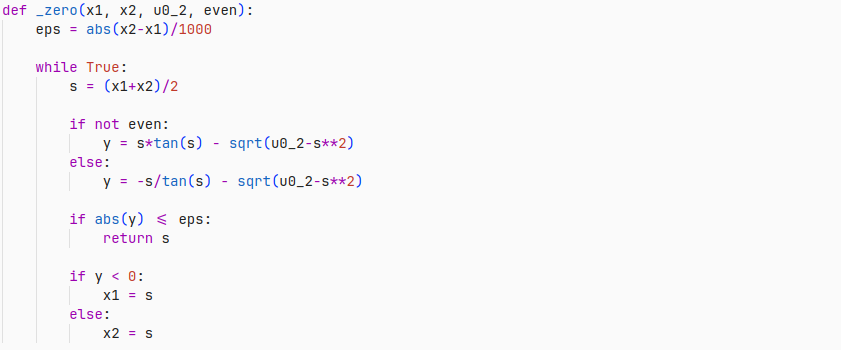
\includegraphics[width=\textwidth,height=\textheight,keepaspectratio]{bisection.png}
		\caption{Implementacja metody bisekcji}
		\label{fig:bisection}
	\end{figure}

Warto jednocześnie zaznaczyć, że wyjątkowej uwagi wymaga znalezienie ostatniego rozwiązania tj. $v_N$. Prawa granica przedziału \ref{v-range}, może być na tyle oddalona od rozwiązania, że wartość z połowy przedziału, liczonej w pierwszej iteracji algorytmu bisekcji, wyniesie więcej niż $u_0$, co spowoduje że w równaniu \ref{eqn:fi-well-vu} pierwiastkowana będzie liczba ujemna. Ponieważ szukane rozwiązania muszą być wartościami rzeczywistymi, przy ostatniej iteracji prawą granicę przedziału, w którym szukane jest miejsce zerowe, ustalam jako $u_0$, co można zobaczyć na rysunku \ref{fig:bisection2}.
	\begin{figure}[H]
		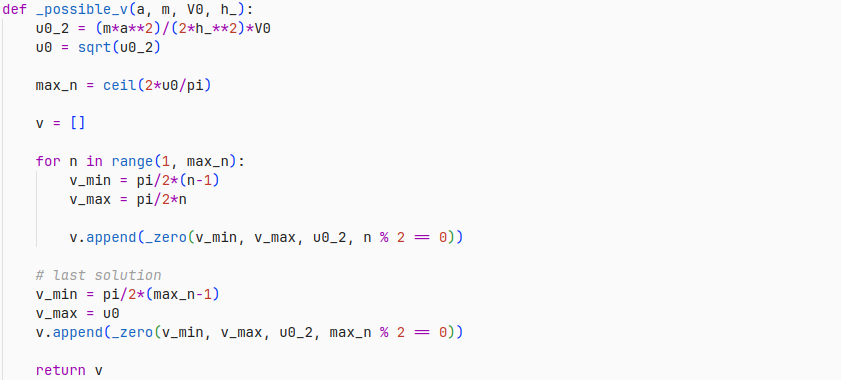
\includegraphics[width=\textwidth,height=\textheight,keepaspectratio]{bisection2.png} 
		\caption{Funkcja znajdująca wszystkie wartości $v$}
		\label{fig:bisection2}
	\end{figure}
	
	Kolejnym nietrywialnym przypadkiem jest obliczenie stałych z układu równań \ref{eqn:barrier-system} dla bariery potencjału. Pomimo że jest to układ liniowy, mnogość wyrazów oraz dziedzina liczb zespolonych powodują, że rozwiązania przyjmują bardzo złożone postacie. Przeglądając literaturę, ciężko doszukać się dokładnych rozwiązań dla każdego z tych współczynników, ponieważ zazwyczaj nie jest to konieczne w rozwiązywaniu praktycznych problemów \cite{fiz atom} \cite{mechanika kwant} \cite{fiz kwant}. Zdecydowałem się więc skorzystać z rozwiązania tego układu numerycznie przy pomocy biblioteki NumPy, co przedstawiłem na rysunku \ref{fig:linalg-solve}
	
	\begin{figure}[H]
		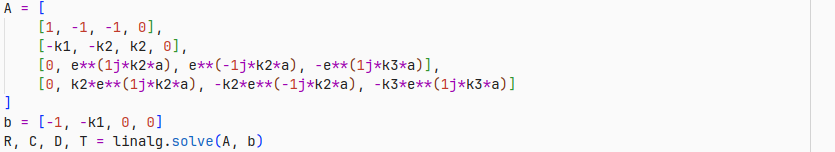
\includegraphics[width=\textwidth,height=\textheight,keepaspectratio]{linalg solve.png} 
		\caption{Implementacja numerycznego rozwiązania układu równań \ref{eqn:barrier-system}}
		\label{fig:linalg-solve}
	\end{figure}

		
	\section{Interfejs pomiędzy językiem TypeScript i Pythonem}
		Języki programowania tak odmienne jak TypeScript i Python uruchamiane są w zupełnie innych środowiskach. Framework Tauri daje tutaj wyjątkową możliwość obsługując język TypeScript przy użyciu WebView \cite{tauri-arch} i Pythona wykorzystująć lokalnie zainstalowany interpreter \cite{tauri-shell}.
		
		Problemem jest jednak przesyłanie danych między tymi językami, o czym nie myślano przy ich tworzeniu. Zastosowałem więc serializację danych do formatu JSON, który jest tekstową reprezentacją obiektu w TypeScript'cie. Wyniki obliczeń fizycznych są więc serializowane w Pythonie jedną z metod na rysunku \ref{fig:to-json}, wysyłane jako wyjście w powłoce systemowej i przekazywane przez Tauri do skryptu napisanego w języku TypeScript przykładowo tak jak na rysunku \ref{fig:ts-run-python}.
		
	\begin{figure}[H]
	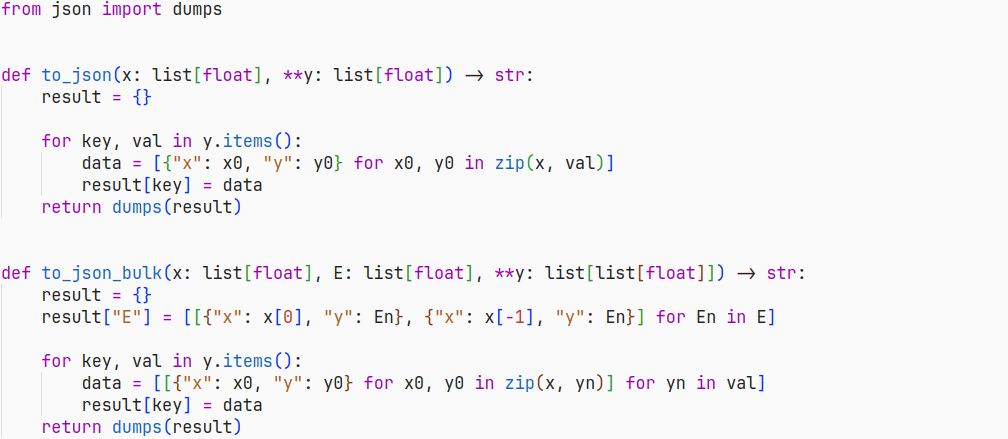
\includegraphics[width=\textwidth,height=\textheight,keepaspectratio]{to_json.png} 
	\caption{Kod z pliku json\_export.py}
	\label{fig:to-json}
	\end{figure}	
	
	\begin{figure}[H]
	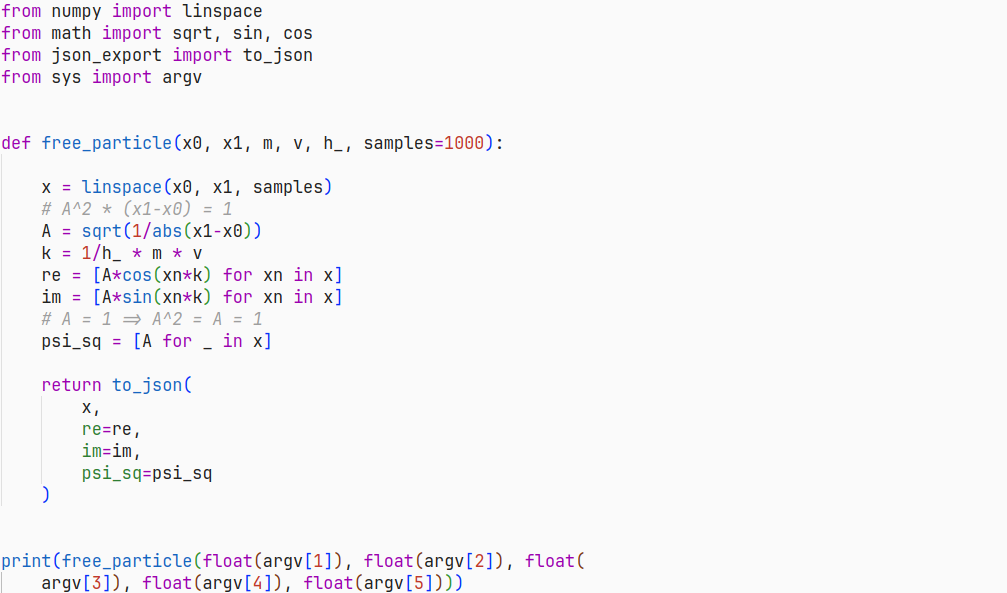
\includegraphics[width=\textwidth,height=\textheight,keepaspectratio]{free_particle py.png} 
	\caption{Wykorzystanie funkcji to\_json w pliku free\_particle.py}
	\label{fig:free-particle-py}
	\end{figure}
	
	\begin{figure}[H]
	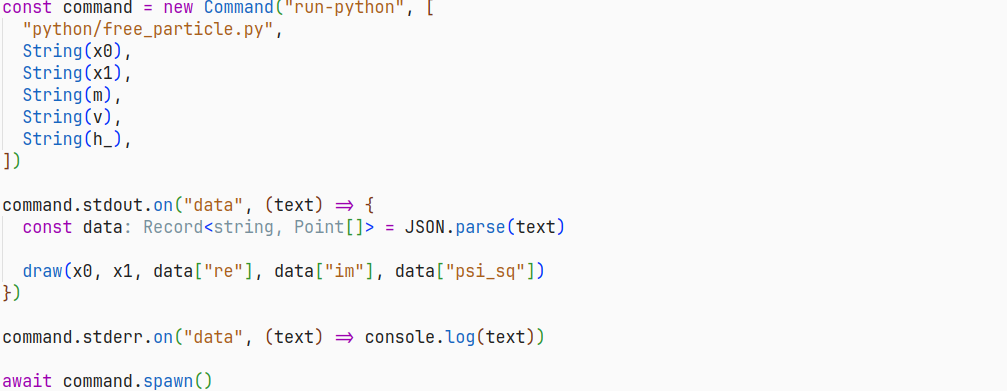
\includegraphics[width=\textwidth,height=\textheight,keepaspectratio]{ts run python.png} 
	\caption{Kod z pliku free-particle.ts}	
	\label{fig:ts-run-python}
	\end{figure}
	
	
	\section{Wdrożenie i dystrybucja aplikacji}
	Aplikacja została stworzona przy użyciu frameworka Tauri, który umożliwia kompilację do formatów .msi i .exe na system Windows, .deb i .AppImage na system GNU/Linux. Możliwa jest też kompilacja na system macOS na architekturę procesora x86 i ARM, jednak nie sprawdzałem tych opcji ponieważ nie mam dostępu do takich urządzeń.
	
	Udostępnione przeze mnie zostały formaty .msi, który w przeciwieństwie do .exe jest dedykowany dla instalatorów programów na system Windows oraz .deb ponieważ jest to format wspierany przez największe dystrybucje systemu GNU/Linux, czyli Debian i Ubuntu. Dodatkowo format .AppImage powodował problem szerzej opisany w kolejnym rozdziale. 
	
	Framework Tauri sam kopiuje do wersji skompilowanej niezbędne pliki .html, .css .ts oraz wszelkie obrazy i fonty użyte w plikach .css, jednak użyte skrypty .py muszą być specjalnie oznaczone jako zasób aplikacji w pliku konfiguracyjnym tauri.conf.json. Ponieważ twórcy frameworka Tauri stworzyli go z myślą o bezpieczeństwie \cite{about-tauri}, w pliku konfiguracyjnym zadeklarować, żeby aplikacja miała możliwość wykonywania poleceń systemowych, do uruchomienia interpretera Pythona oraz możliwość odczytu plików, do użycia plików ze skryptami Pythona.
	
	Ponieważ obliczenia matematyczne wykonywane są przy użyciu języka Python, niezbędny do działania aplikacji jest zainstalowany interpreter Pythona 3.11 lub nowszy z zainstalowanym modułem NumPy. Zdecydowałem się nie dołączać interpretera do instalatora mojej aplikacji, ponieważ znacząco zwiększyłoby to rozmiar finalnego pliku. 
	\section{Problemy, ograniczenia i możliwości rozwoju}
	Jedno z ważniejszych ograniczenie mojej aplikacji leży w interfejsie pomiędzy językiem TypeScript i Pythonem. O ile wykonanie samych obliczeń fizycznych w Pythonie liczyć można w milisekundach to proces zserialozwania danych, przekazania ich do odczytu i deserializacji w języku TypeScript wydłuża ten proces do kilkuset milisekund, zwykle co najmniej 200. Jest to czas niezauważalny jeżeli potrzebne jest wykonanie obliczeń raz lub stosunkowo rzadko, co ma miejsce w aplikacji, jednak częste odświeżanie wyświetlanych danych byłoby po prostu niemożliwe do zrealizowania, przy zastosowanym rozwiązaniu. Należy jednocześnie zwrócić uwagę, że przy bardziej rozbudowanych scenariuszach fizycznych czas przekazywania danych może okazać się nieznaczący, jeśli samo wykonywanie obliczeń fizycznych trwać znacznie dłużej. Dokładnie takie przypadki miałem na względzie decydując o zastosowaniu Pythona w projekcie i jest to kierunek, w którym aplikacja mogłaby zostać w przyszłości rozwinięta.
	
	Kolejną rzeczą, która ogranicza aplikację jest forma dystrybucji. Na przestrzeni lat aplikacje desktopowe ustępowały popularnością aplikacjom webowym \cite{web-vs-desktop}. W wyniku takich zmian użytkownicy przyzwyczajeni do korzystania z przeglądarki internetowej mogą nie chcieć poświęcić czasu na pobranie i zainstalowanie mojej aplikacji. Niestety jednak, pomimo że jest to już możliwe, wykonywanie skryptów Pythona w przeglądarce jest dalej w fazie rozwoju \cite{python-webassembly} co wymusza taką formę aplikacji.
	
	Z pozoru największym problemem jaki napotkałem był fakt, że aplikacja po skompilowaniu do formatu .AppImage nie była w stanie poprawnie wywoływać skryptów Pythona. Jak jednak powiedziałem, problem tylko z pozoru wydał się krytyczny, a to przez fakt, że formaty .deb i .msi nie sprawiały żadnych problemów. Wciąż zaintrygowany tym nieoczekiwanym zachowaniem, zgłosiłem się przez komunikator Discord o pomoc do zespołu wsparcia frameworka Tauri. Okazało się, że nie jest to spodziewane zachowanie i najprawdopodobniej napotkałem błąd w samym frameworku. Za prośbą zespołu wsparcia zamieściłem repozytorium z minimalnym kodem niezbędnym do odtworzenia tego błędu \cite{app-error-repo}.
	
	Ważnym aspektem, który niekiedy spowalniał tworzenie pracy, jest fakt że framework Tauri, wydany w 2022 roku \cite{tauri-release}, jest stosunkowo nową technologią. Pomimo że dostępną jest dokumentacja, to potrafi ona zawierać braki lub niedopowiedzenia, a szukanie szczegółowych odpowiedzi może stanowić wyzwanie, ponieważ nie istnieje na ten temat znacząca ilość literatury.
	
	Rzeczą którą niewątpliwie można poprawić, jednak nie jest ona moim zdaniem kluczowa, jest weryfikacja instalacji interpretera języka Python. Aktualnie aplikacja nie weryfikuje czy interpreter ten jest rzeczywiście zainstalowany oraz czy zainstalowany jest moduł NumPy. Dodanie takiej funkcjonalności w przyszłości niewątpliwie pomogłoby, w szukaniu problemów w razie nieprawidłowego działania aplikacji.
	

\chapter{Interfejs aplikacji}
	\section{Ekran główny}
	\section{Interaktywna wizualizacja}
	\section{Narrator}
	
\chapter{Podsumowanie i wnioski}


\begin{thebibliography}{9}
	\bibitem{fiz atom}
	M.R. Wehre, H.A. Enge, J.A. Richards,
	\textit{Wstęp do fizyki atomowej}, 
	Państwowe Wydawnictwo Naukowe, Warszawa 1983. ISBN 83-01-02200-0
	
	\bibitem{mechanika kwant}
	L.D. Landau, E.M. Lifszyc,
	\textit{Mechanika kwantowa Teoria nierelatywistyczna}
	Państwowe Wydawnictwo Naukowe, Warszawa 1979. ISBN 83-01-00501-7
	
	\bibitem{fiz kwant}
	R. Eisberg, R. Resnick,
	\textit{Fizyka kwantowa atomów, cząsteczek, ciał stałych, jąder i cząstek elementarnych}
	Państwowe Wydawnictwo Naukowe, Warszawa 1983. ISBN 83-01-04350-1

	\bibitem{JS}
	David Flanagan, 
	\textit{JavaScript: The Definitive Guide. Master the World's Most-Used Programming Language. 7th Edition}, 
	O'Reilly Media, 2020. ISBN 978-14-919-5198-9
	
	\bibitem{Python}
	Wes McKinney,
	\textit{Python for Data Analysis}
	O'Reilly Media, 2012. ISBN 078-1-449-31979-3
	
	\bibitem{chartjs}
	Dokumentacja Chart.js
	\textit{https://www.chartjs.org/docs/latest/}
	(ostatni dostep 30.04.2024)
	
	\bibitem{about-tauri}
	Prezentacja Tauri
	\textit{https://tauri.app/about/intro}
	(ostatni dostęp 28.04.2024)
	
	\bibitem{sympy}
	Dokumentacja SymPy
	\textit{https://docs.sympy.org/latest/index.html}
	(ostatni dostęp 13.01.2024)
	
	\bibitem{nuclear-stats}
	Statystyki eurostat na temat energetyki jądrowej
	\textit{https://ec.europa.eu/eurostat/statistics-explained/index.php?title=Nuclear\_energy\_statistics}
	(ostatni dostęp 28.04.2024)
	
	\bibitem{foto-ele}
	Wikipedia, efekt fotoelektryczny 
	\textit{https://pl.wikipedia.org/wiki/Efekt\_fotoelektryczny}
	(ostatni dostęp 15.01.2024)
	
	\bibitem{matter-wave}
	Wikipedia, fale materii
	\textit{https://pl.wikipedia.org/wiki/Fale\_materii}
	(ostatni dostęp 15.01.2024)
	
	\bibitem{schrodinger-equation}
	Wikipedia, równanie Schrödingera
	\textit{https://pl.wikipedia.org/wiki/Równanie\_Schrödingera}
	(ostatni dostęp 15.01.2024)
	
	\bibitem{wikipedia-well}
	Wikipedia, studnia kwantowa
	\textit{https://pl.wikipedia.org/wiki/Studnia\_kwantowa}
	(ostatni dostęp 15.01.2024)
	
	\bibitem{newton-method}
	Wikipedia, metoda Newtona
	\textit{https://pl.wikipedia.org/wiki/Metoda\_Newtona}
	(ostatni dostęp 15.01.2024) 
	
	\bibitem{bisection-method}
	Wikipedia, metoda równego podziału
	\textit{https://pl.wikipedia.org/wiki/Metoda\_równego\_podziału}
	(ostatni dostep 15.01.2024)
	
	\bibitem{tauri-arch}
	Architektura Tauri
	\textit{https://tauri.app/v1/references/architecture/}
	(ostatni dostęp 28.04.2024)
	
	\bibitem{tauri-shell}
	Dokumentacja API shell w Tauri
	\textit{https://tauri.app/v1/api/js/shell/}
	(ostatni dostęp 28.04.2024)
	
	\bibitem{web-vs-desktop}

	
	\bibitem{python-webassembly}
	Repozytorium Pyodide
	\textit{https://github.com/pyodide/pyodide}
	(ostatni dostęp 28.04.2024)
	
	\bibitem{app-error-repo}
	Repozytorium do odtworzenia błędu w kompilacji aplikacji Tauri do AppImage
	\textit{https://github.com/xAdiro/tauri-appimage-python-error}
	(ostatni dostęp 28.04.2024)
	
	\bibitem{tauri-release}
	Plan działania Tauri 2.0
	\textit{https://beta.tauri.app/blog/roadmap-to-tauri-2-0/}
	(ostatni dostęp 28.04.2024)
	
	
	
	
	
	
	
	
	
\end{thebibliography}

\beforelastpage

\end{document}
